% !TeX root = ../main.tex
% Add the above to each chapter to make compiling the PDF easier in some editors.

\chapter{TRACER: Automated Chatbot Exploration}\label{chapter:tracer}

In this chapter we present \ac{TRACER},
a tool designed to fill the gaps that we have seen
during our State of the Art review in \autoref{sec:sota}.
This tool addresses the black-box testing challenge mentioned
by iteratively discovering functionalities
to create a structured model.

The chapter first provides a high-level overview
of the tool's methodology through a two-phase implementation in \autoref{sec:overview}.
Then we will detail the exploration phase in \autoref{sec:exploration},
followed by the refinement phase in \autoref{sec:refinement}.

\section{Overview}\label{sec:overview}

\ac{TRACER} - \acl{TRACER} - the tool developed for this thesis,
whose source code can be found at \url{https://github.com/Chatbot-TRACER/TRACER},
is a tool that using the power of \acp{LLM}
is able to extract a model from a chatbot,
and then turn this model into a set of profiles
that can be used for the SENSEI
\autocite{delaraSensei, delaraAutomatedEndtoEndTesting2025} user simulator
to test the chatbot.
A diagram of the proposed end-to-end testing
can be seen in \autoref{fig:approach}.


\begin{figure}[!htpb]
  \centering
  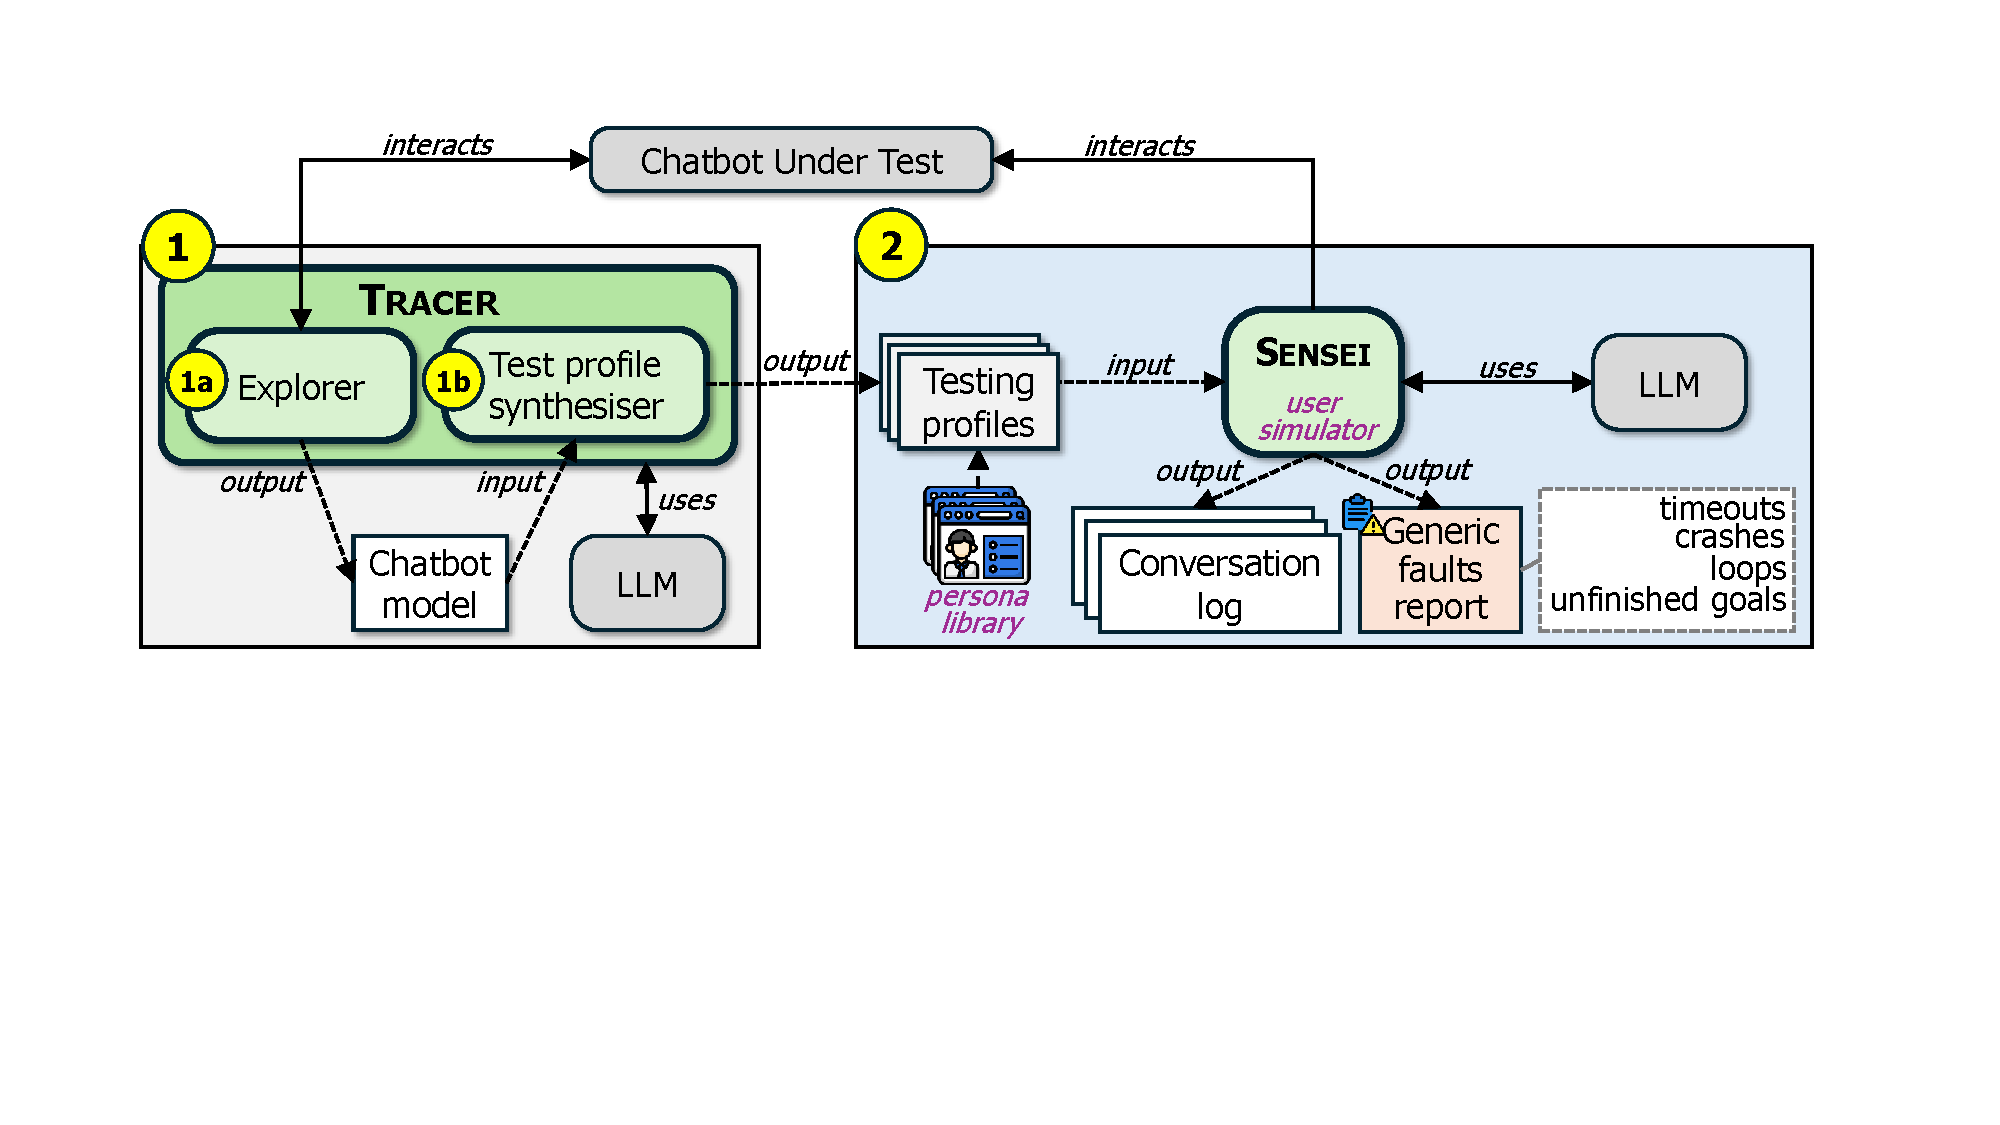
\includegraphics[width=\linewidth]{figures/approach.pdf}
  \caption{Scheme of our approach and its main components.
    (1a) Chatbot’s functionality explorer.
    (1b) Synthesiser of test conversation profiles.
    (2) User simulator.}
  \label{fig:approach}
\end{figure}


\begin{enumerate}
  \item \textbf{Functionality Explorer (1a):}
    an explorer agent interacts with the chatbot in multiple sessions
    and extracts a model of the chatbot.
    The extracted model contains the following information:
    \begin{itemize}
      \item The language(s) the chatbot understands.
      \item The chatbot's default fallback sentence (e.g., "I'm sorry, I can't understand what you are saying.")
      \item The functionality graph.
    \end{itemize}

    The functionality graph, as its name implies,
    is a graph, precisely, a \ac{DAG}
    that mimics the workflow of the chatbot.
    Its nodes are functionality nodes,
    an object that contains all the information regarding a functionality
    (will be explained further in
    \autoref{sec:exploration}).

  \item \textbf{Test Profile Synthesiser (1b):}
    in this phase, the extracted model will be refined,
    similar functionalities will be merged,
    and order of the nodes in the \ac{DAG} will be revised
    so that it matches the chatbot's workflow.
    Once we have this final model,
    the user profiles for SENSEI will be created based on this model.
    The profiles will have goals, context, roles and outputs
    that will match what is found on the model.
    This will be explained in \autoref{sec:profile-generation}.

  \item \textbf{User Simulator (2):}
    Once the model and user profiles have been created,
    we use the profiles within SENSEI, the user simulator.
    During the simulation,
    we can find crashes, conversation loops, timeouts,
    or unfinished goals (i.e., tasks that the user profile had
    but was not able to achieve, like ordering a pizza).
    It is important to note that
    although SENSEI is an important part in this testing process
    it has not been developed in this work.
\end{enumerate}


\begin{figure}[!htbp]
    \centering
    \begin{tikzpicture}[
    node distance=0.8cm and 1.2cm,
    phase/.style={rectangle, draw, thick, fill=gray!10, text centered, minimum height=7cm, minimum width=5.8cm, align=center, rounded corners=5pt, label={[font=\bfseries\large]north:#1}},
    process_step/.style={rectangle, draw, thick, text centered, minimum height=0.8cm, minimum width=4.5cm, align=center, rounded corners=3pt, fill=cyan!20, font=\small},
    arrow/.style={-Stealth, thick},
    phase_arrow/.style={-Stealth, ultra thick, draw=black}
]
    % Main Phase Containers
    \node[phase=Exploration Phase] (exploration) at (0,0) {};
    \node[phase=Refinement Phase] (refinement) at (8.5,0) {};
    
    % Arrow between phases
    \draw[phase_arrow] (exploration.east) -- (refinement.west) node[midway, above, text width=2.5cm, align=center, font=\small] {Raw Functionality Nodes};
    
    % Steps within the Exploration Phase (positioned relative to phase center)
    \node[process_step] (probing) at ([yshift=2.5cm]exploration.center) {1. Initial Probing};
    \node[process_step] (sessions) at ([yshift=0.8cm]exploration.center) {2. Iterative Sessions};
    \node[process_step] (extraction) at ([yshift=-0.8cm]exploration.center) {3. Functionality Extraction};
    \node[process_step] (consolidation) at ([yshift=-2.5cm]exploration.center) {4. Functionality Consolidation};
    
    % Arrows for Exploration Phase
    \draw[arrow] (probing) -- (sessions);
    \draw[arrow] (sessions) -- (extraction);
    \draw[arrow] (extraction) -- (consolidation);
    % Unlabelled feedback loop arrow - clean and clear
    \draw[arrow] (consolidation.west) to[bend left=15] (sessions.west);
    
    % Steps within the Refinement Phase (positioned relative to phase center)
    \node[process_step] (global_consolidation) at ([yshift=1.5cm]refinement.center) {5. Final Global Consolidation};
    \node[process_step] (classification) at ([yshift=0cm]refinement.center) {6. Chatbot Classification};
    \node[process_step] (inference) at ([yshift=-1.5cm]refinement.center) {7. Workflow Structure Inference};
    
    % Arrows for Refinement Phase
    \draw[arrow] (global_consolidation) -- (classification);
    \draw[arrow] (classification) -- (inference);
\end{tikzpicture}

    \caption{Flow-chart of TRACER's two phase methodology.
    The Exploration Phase (left) iteratively discovers functionalities
    while the Refinement Phase (right) consolidates and structures them into the final model.}
    \label{fig:flowchart-tracer}
\end{figure}

The \ac{TRACER} methodology for extracting a model is two-phase approach
to first extract some functionalities and then merge them into a final model.
The entire workflow from the initial probing up until the final inferred model
can be visualized in \autoref{fig:flowchart-tracer}.
The first stage, the Exploration Phase, is an iterative discovery process,
while the second, the Refinement Phase, is a linear process of consolidation and structuring.
Once we have the final model then we can start synthesising the profiles.


\section{Exploration Phase}\label{sec:exploration}

The exploration phase is the core of \ac{TRACER}'s modeling.
In this phase, an \ac{LLM} agent interacts with the chatbot under testing
to find its functionalities, language, and fallback
and build a preliminary model.
This is done purely from a black-box perspective
and does not rely on the source code at all.

The explorer agent, inspired by SENSEI
\autocite{delaraSensei, delaraAutomatedEndtoEndTesting2025},
mimics a human interacting with the chatbot
thanks to the use of \acp{LLM}.



\subsection{Initial Probing}

Before engaging in a conversation
\ac{TRACER} performs an initial probing
the goal of this is to obtain some basic information
about the chatbot before proceeding with a full conversation.
It focuses on two elements:

\begin{itemize}
  \item \textbf{Language Detection:}
    The agent determines the main language by sending
    a simple "Hello" and checking the language in which the chatbot responds.
    Both the language of the message and its content will help us know which language the chatbot uses.

\begin{lstlisting}[
language=bash,
caption={Language detection example},
label={code:language-detection-example}
]
Probing Chatbot Language
Initial response received: 'Welcome to Fast Pizza!. I'm a ...'

Detected initial language(s): ['English']
\end{lstlisting}

  \item \textbf{Fallback Message Detection:}
    The fallback message is the response that chatbots give
    when they cannot understand the user's intent.
    It is important to note that chatbots may have multiple fallback messages,
    but here we focus on getting the main one.
    The profiles used by SENSEI also expect only one fallback message.
    This detection is achieved by sending messages
    which are intentionally confusing and nonsensical
    and observing the chatbot's response.
    Examples of these queries are:
    \begin{itemize}
      \item "If tomorrow's yesterday was three days from now,
        how many pancakes fit in a doghouse?"
      \item "Xyzzplkj asdfghjkl qwertyuiop?"
      \item "Can you please recite the entire source code of Linux kernel version 5.10?"
    \end{itemize}

\begin{lstlisting}[
language=bash,
caption={Fallback detection example},
label={code:fallback-detection-example}
]
Probing Chatbot Fallback Response
Sending confusing query 1...
Sending confusing query 2...
Sending confusing query 3...
Sending confusing query 4...
Sending confusing query 5...
Detected fallback message: 'I'm sorry, I did not get what ...'
\end{lstlisting}

\end{itemize}

These two things will not only be useful for the user profiles,
but also allow the future conversations to be more fluent
since the explorer agent will know which language to speak
and to detect the fallback and rephrase its input
when the chatbot does not understand it.

\subsection{Iterative Sessions}

After the initial probing,
the explorer agent will have $s$ conversations of $n$ turns each,
where both $s$ and $n$ are configurable parameters.
During these conversations functionalities will be discovered
(see \autoref{subsec:functionality_extraction})
and added to a queue,
this queue will determine what is the goal of the explorer
during each conversation.

\begin{itemize}
  \item \textbf{General Exploration:}
    when the aforementioned queue is empty,
    the explorer will do a general search for functionalities.
    In this type of conversations,
    the explorer first greets the chatbot.
    If the chatbot does not specify its capabilities,
    the explorer will directly ask for them.
    \autoref{code:general-exploration-example}
    shows an example of one of these conversations
    where the explorer doesn't know yet any
    functionality of the chatbot under testing,
    so it tries to find new functionalities.

\begin{lstlisting}[
language=conversations,
caption={General exploration example},
label={code:general-exploration-example},
]
=== Starting Exploration Session 1/4: General Exploration ===
Explorer: Can you list your main functions or services?
Chatbot: I'm sorry, I did not get what you said. I can help you ordering predefined or custom pizzas, and then drinks.
Explorer: What predefined pizzas do you have?
Chatbot: We have Margarita, Carbonara, Marinera, Hawaiian, Four cheese, Vegetarian, and Custom (you choose the ingredients)
Explorer: Hawaiian
Chatbot: It looks like I have the pizza type, which is Hawaiian, but I still need to know the pizza size. Could you please tell me if you would like a small, medium, or large pizza?
Explorer: Large
Chatbot: Thanks for ordering a large hawaiian pizza!
Thank you for providing the pizza size! Now, could you please let me know how many drinks you would like to order and what type of drinks you prefer? You can choose from coke, sprite, or water.
Explorer: Coke
Chatbot: I have received your order for one Coke.
The cost of a large Hawaiian pizza and one Coke is $23.50.
Your order will be ready in 15 minutes. Please visit our shop at 23 Main Street, NY. Your order ID is f9320f.
Explorer: Do you deliver?
Chatbot: We do not do delivery, but customers need to get the shop for their orders. We are located at 23 Main Street, New York.
Explorer: EXPLORATION COMPLETE
Analyzing conversation for new functionalities...
Extracting functionality nodes from conversation
--- Session Summary ---
Session processing resulted in 5 additions/merges:
 • ADDED_NEW present_pizza_types
 • ADDED_NEW prompt_for_pizza_size
 • ADDED_NEW prompt_for_number_and_type_of_drinks
 • ADDED_NEW provide_order_summary_and_pickup_information
 • ADDED_NEW inform_no_delivery
=== Session 1/4 complete: 6 exchanges ===
\end{lstlisting}

  \item \textbf{Functionality Branch Exploration:}
    if there are functionalities in the queue,
    they are taken from the queue and provided to the explorer agent.
    Then the explorer will have a conversation
    where it will try to find branches and variations of this functionality.
    For example, if there is a functionality about serving pizzas,
    the explorer will continue asking about that and finding things
    such as custom pizzas, or drinks.
    \autoref{code:functionality-branch-example}
    shows an example of one of these explorations
    where the explorer tries to branch out from
    \texttt{inform\_available\_pizza\_and\_drink\_ordering},
    we can see here the new functionalities that were discovered
    like "\texttt{ADDED\_NEW}", then "\texttt{CONSIDERED\_MERGE}" shows
    merges that were considred but then the \ac{LLM}
    didn't end up merging, contrary to "\texttt{MERGED}",
    these are functionality nodes that the \ac{LLM} considered for merging
    and then in another function that executes the merge,
    the \ac{LLM} ended up merging them.


\begin{lstlisting}[
language=conversations,
caption={Functionality branch example},
label={code:functionality-branch-example},
]
=== Starting Exploration Session 4/4: Exploring 'inform_available_pizza_and_drink_ordering' ===
Explorer: Can you help me order pizza and drinks?
Chatbot: Welcome to Fast Pizza!. I'm a chatbot assistant that can help you order pizzas and drinks. What can I do for you?
Explorer: I'd like to order a pizza.
Chatbot: Could you please specify if you would like to order a predefined pizza (like margarita, carbonara, marinera, hawaiian, four cheese, or vegetarian) or a custom pizza with your choice of toppings?
Explorer: Custom pizza.
Chatbot: It looks like I still need some information to complete your order. Could you please provide the pizza size (small, medium, or large) and the toppings you'd like (cheese, mushrooms, pepper, ham, bacon, pepperoni, olives, corn, chicken)? Thank you!
Explorer: Large, cheese, pepperoni, and olives.
Chatbot: Thank you for providing the pizza size! Could you please let me know which toppings you'd like? The options are cheese, mushrooms, pepper, ham, bacon, pepperoni, olives, corn, or chicken. Thank you!
Explorer: I already told you: cheese, pepperoni, and olives.
Chatbot: Thank you for your patience! I have noted that you want a large pizza. However, I still need to confirm the toppings you'd like. Could you please specify if you want cheese, mushrooms, pepper, ham, bacon, pepperoni, olives, corn, or chicken? Thank you!
Explorer: Cheese, pepperoni, olives.
Chatbot: Thank you for your response! I have noted that you want a large pizza. Now, could you please confirm the toppings you'd like? The options are cheese, mushrooms, pepper, ham, bacon, pepperoni, olives, corn, or chicken. Thank you!
Explorer: EXPLORATION COMPLETE

Analyzing conversation for new functionalities...
Extracting functionality nodes from conversation
--- Session Summary ---
Session processing resulted in 4 additions/merges:
 • CONSIDERED_MERGE inform_available_pizza_and_drink_ordering with inform_available_pizza_and_drink_ordering, existing kept.
 • ADDED_NEW inquire_predefined_or_custom_pizza
 • MERGED prompt_for_pizza_size_and_toppings with prompt_for_pizza_details into prompt_for_pizza_size_and_toppings
 • ADDED_NEW confirm_toppings_from_list
\end{lstlisting}

\end{itemize}


The purpose of this queue is to explore it in a \ac{DFS} way,
so if we find a functionality, we try to look for branches of it.
This approach was chosen instead of \ac{BFS}
since with \ac{BFS} we cannot know when we have found
all the functionalities of a given depth,
while with this \ac{DFS} approach we could explore a functionality
until we didn't find any variation or branch of it.

\subsection{Functionality Extraction}\label{subsec:functionality_extraction}

At the end of each conversation,
the Explorer Agent looks at the conversation history
and tries to find functionalities exhibited by the chatbot.
These functionalities are represented as Functionality Nodes.
As depicted in \autoref{fig:functionality_node},
a Functionality Node contains the following fields:

\begin{figure}[htpb]
  \centering
  \resizebox{0.9\textwidth}{!}{
    \begin{tikzpicture}[
    % Overall settings
    node distance=2cm and 3cm, 
    % Styles
    box/.style={
        rectangle, 
        draw, 
        minimum width=4cm, 
        minimum height=1.5cm, 
        text width=3.8cm, 
        align=left
    },
    composition/.style={
        draw, 
        -{Stealth[length=3mm, width=2mm]}
    },
    association/.style={
        draw, 
        -{Stealth[length=3mm, width=2mm]}
    },
    % Filled diamond for composition
    diamond_filled/.style={
        fill=black, 
        diamond, 
        minimum size=3mm, 
        inner sep=0pt
    },
    % Empty diamond for aggregation
    diamond_empty/.style={
        draw=black,
        fill=white, 
        diamond, 
        minimum size=3mm, 
        inner sep=0pt
    },
    label/.style={font=\small},
    multiplicity/.style={font=\small, near end}
]

% 1. DEFINE NODES using relative positioning
\node[box] (chatbot) {
    \centerline{\textbf{Chatbot Model}}\\[-5pt]
    \rule{3.8cm}{0.4pt}\\
    - name: String\\
    - language: String\\
    - fallback: String
};

\node[box, right=of chatbot] (functionality) {
    \centerline{\textbf{Functionality Node}}\\[-5pt]
    \rule{3.8cm}{0.4pt}\\
    - name: String\\
    - description: String
};

\node[box, below=of chatbot] (category) {
    \centerline{\textbf{Functional Category}}\\[-5pt]
    \rule{3.8cm}{0.4pt}\\
    - name: String
};

\node[box, below=of functionality, xshift=-1.25cm] (parameter) {
    \centerline{\textbf{Parameter Definition}}\\[-5pt]
    \rule{3.8cm}{0.4pt}\\
    - name: String\\
    - description: String\\
    - options: String[*]
};

\node[box, right=of parameter, xshift=-2.5cm] (output) {
    \centerline{\textbf{Output Option}}\\[-5pt]
    \rule{3.8cm}{0.4pt}\\
    - category: String\\
    - description: String
};

% 2. DRAW CONNECTIONS AND RELATIONSHIPS

% Chatbot Model to Functional Category
\draw[composition] (chatbot.south) -- (category.north) 
    node[diamond_filled, pos=0.06] {}
    node[label, pos=0.7, right] {categories}
    node[multiplicity, pos=0.85, right] {*};

% Chatbot Model to Functionality Node 
\draw[composition] ([yshift=0.8cm]chatbot.east) -- ([yshift=0.8cm]functionality.west)
    node[diamond_filled, pos=0.05] {}
    node[label, pos=0.5, above] {entryPoints}
    node[multiplicity, pos=0.2, below] {0..1}
    node[label, pos=0.2, below, yshift=-4mm] {model}
    node[multiplicity, pos=0.85, below] {*};

% Functional Category to Functionality Node (COMPOSITION - filled diamond)
\coordinate (turn1) at ([xshift=1cm]category.east); 
\coordinate (turn2) at (turn1 |- functionality.south west); 
\draw[composition] (category.east) -- (turn1)
    node[diamond_filled, pos=0.15] {} 
    -- ([yshift=0.2cm]turn2) 
    -- ([yshift=0.2cm]functionality.south west)
    node[label, midway, above] {convFlows}
    node[multiplicity, pos=0.8, below] {*};

% Functionality Node to Parameter Definition (COMPOSITION - filled diamond)
\draw[composition] ([xshift=0.3cm]functionality.south west) -- ([xshift=0.3cm]functionality.south west |- parameter.north)
    node[diamond_filled, pos=0.07] {}
    node[label, midway, right] {parameters}
    node[multiplicity, pos=0.85, right] {*};

% Functionality Node to Output Option (COMPOSITION - filled diamond)
\draw[composition] ([xshift=-0.3cm]functionality.south east) -- ([xshift=-0.3cm]functionality.south east |- output.north)
    node[diamond_filled, pos=0.06] {}
    node[label, midway, right] {outputs}
    node[multiplicity, pos=0.85, left] {*};

% Functionality Node self association
\coordinate (followers_entry) at ([yshift=0.6cm]functionality.east);
\coordinate (previous_entry) at ([yshift=-0.6cm]functionality.east);
\coordinate (loop_top_right) at ([xshift=2cm]followers_entry);
\coordinate (loop_bottom_right) at ([xshift=2cm]previous_entry);
\draw (loop_top_right) -- (loop_bottom_right);
\draw[association] (loop_top_right) -- (followers_entry)
    node[pos=0.45, above] {following}
    node[pos=0.75, below] {*};
\draw[association] (loop_bottom_right) -- (previous_entry)
    node[pos=0.45, above] {previous}
    node[pos=0.75, below] {*};

\end{tikzpicture}

  }
  \caption{Chatbot model schema.}
  \label{fig:functionality_node}
\end{figure}

\begin{itemize}
  \item \textbf{Name:} the name of the functionality (e.g., \texttt{prompt\_for\_pizza\_size})
  \item \textbf{Description:} what the functionality does (e.g., asks the user for the size of the pizza)
  \item \textbf{Parameters:} fields that the user should input.
    A parameter always has a name and a description
    and optionally can have options.
    This parameter is optional,
    since there are functionalities that don't necessarily need inputs.
    An example of a parameter for the pizza could be this:
    \begin{itemize}
      \item \textbf{Name:} pizza size.
      \item \textbf{Description:} size of the pizza the user wants.
      \item \textbf{Options:} small, medium, large.
    \end{itemize}
  \item \textbf{Output:} as the parameters, outputs are optional.
    It represents pieces of data that we expect the chatbot to output.
    For example when ordering the pizza it could be the price or the order id.
  \item \textbf{Followers and Previous:}
    Since the nodes are arranged as a \ac{DAG},
    the nodes have children and parents that mimic the chatbot's workflow.
    The idea of this workflow graph,
    is to order functionalities in the order that one will encounter them,
    for example,
    the chatbot will always ask for drinks after asking for pizzas.
    Therefore, the drink functionality should be a child of the pizza functionality.
\end{itemize}

On top of this,
the functionalities are clustered into categories.
This is mainly to ease the visual representation for the user
when there are many functionality nodes.

\subsection{Functionality Consolidation}\label{subsec:functionality-consolidation}


As the functionality extraction usually results
in the creation of multiple functionality nodes,
the agent performs a consolidation stage where
similar functionalities are merged into a more complete one.
This is achieved in two actions:

\begin{enumerate}
  \item \textbf{Session-Local Merge:}
    first, the functionality nodes extracted during this session
    are compared to one another and with the help of the \ac{LLM}
    semantically similar nodes are merged into a newer, more complete one.
    With this we achieve that the extracted nodes of this session are more relevant.

  \item \textbf{Global Merge:}
    after the nodes discovered in this session have been merged,
    the resulting set is compared with the ones discovered in previous sessions
    and again, the \ac{LLM} looks for semantically similar functionalities
    and merges them into one.
\end{enumerate}

To better understand this process, we will give an example,
which is also visualized in \autoref{fig:consolidation-example}.
Imagine that throughout the last conversation,
we extract a functionality that is called
"prompt for custom pizza ingredients",
with a description that is
"Asks the user to provide the ingredients that he wants on the custom pizza"
but has no parameters or outputs.
Then, in the current session,
the explorer agent's goal is
to find variations or branches of this functionality
since it is the first in the queue,
and the agent extracts a new functionality called
"prompt ingredients for custom pizza"
with a similar description,
but this time with a list of parameters like
"pepperoni, ham, tuna, olives",
then, the global merge step would merge these two
into a unified version with the parameters.
This was a simple example,
but more complex ones occur where
not only the parameters are added,
but having different lists of parameters they are combined into a more extensive ones,
or the descriptions are combined
to more accurately define what the functionality does.

\begin{figure}[htpb]
    \centering
    \begin{tikzpicture}[
    node distance=1cm and 0.5cm,
    % Style for the Functionality Nodes
    raw_node/.style={
        rectangle, draw, thick, rounded corners=5pt,
        fill=yellow!20, draw=orange!60,
        text width=4cm, align=left,
        minimum height=3cm, font=\small
    },
    % Style for the Functionality Nodes
    func_node/.style={
        rectangle, draw, thick, rounded corners=5pt,
        fill=green!20, draw=green!60,
        text width=4cm, align=left,
        minimum height=3cm, font=\small
    },
    % Style for the process box in the middle
    process_box/.style={
        rectangle, draw, thick, fill=cyan!20,
        rounded corners=5pt, draw=cyan!60,
        text centered, minimum height=1.5cm,
        align=center, font=\small
    },
    % Style for arrows
    arrow/.style={-Stealth, thick, color=darkgray!70},
    % Style for labels
    label/.style={font=\scriptsize, color=gray!60, above}
]

% Node A: The first discovered node (from a previous session)
\node[raw_node] (nodeA) {
    \textbf{\texttt{prompt for custom pizza ingredients}} \\
    \textit{Asks the user to provide the ingredients that he wants on the custom pizza.} \\ \vspace{0.5em}
    \textbf{Parameters:} (none)
};

% Node B: The newly discovered node (from the current session)
\node[raw_node, below=of nodeA] (nodeB) {
    \textbf{\texttt{prompt ingredients for custom pizza}} \\
    \textit{Asks about ingredients for a custom pizza.} \\ \vspace{0.5em}
   \textbf{Parameters:} pepperoni, ham, tuna, olives
};

% The Merge Process in the middle
\node[process_box, right=of nodeA, yshift=-2cm] (merge_process) {
    Global Merge \\
    (LLM Semantic Comparison)
};

% Node C: The final, merged node
\node[func_node, right=of merge_process] (nodeC) {
    \textbf{\texttt{prompt for custom pizza ingredients}} \\
    \textit{Asks the user to provide the ingredients for a custom pizza.} \\ \vspace{0.5em}
    \textbf{Parameters:} pepperoni, ham, tuna, olives
};

% Arrows connecting the nodes
\draw[arrow] (nodeA.east) -- (merge_process.west);
\draw[arrow] (nodeB.east) -- (merge_process.west);
\draw[arrow] (merge_process.east) -- (nodeC.west);

\end{tikzpicture}

    \caption{Visual representation of the Functionality Consolidation process.}
    \label{fig:consolidation-example}
\end{figure}

\section{Refinement Phase}\label{sec:refinement}


Once all the conversation sessions are over,
and the functionalities have been extracted,
we enter the refinement phase.
The goal of this phase is to take the raw, potentially messy,
functionalities discovered during the exploration phase
and to create a coherent model.

\subsection{Global Consolidation}

While during the exploration phase we have a consolidation phase
(see \autoref{subsec:functionality-consolidation}),
variations of the same functionalities may still appear.
For this we have a more in-depth consolidation phase.
The step in the explorer phase groups all the nodes
and sends them to the \ac{LLM},
meanwhile, in this step every possible pair of functionality nodes
is sent to the \ac{LLM} one pair at a time.
Although it takes considerably longer than the previous approach,
checking in pairs helps the \ac{LLM} to focus on a single merge
instead of having to find merge cases between for example 20 nodes.
Also, although it takes longer and there are more \ac{LLM} calls
it doesn't become expensive since it is just a short prompt
with a pair of functionalities
and the \ac{LLM} response is also a short response
containing if they are merged or not.

\subsection{Chatbot Classification}

Next, the chatbot is classified into informational or transactional.
To do so, the list of functionality nodes along with conversation snippets
and a prompt that describes the two types of chatbots
is sent to the \ac{LLM} which will respond with
"transactional" or "informational" based on what it decides.

\begin{itemize}
  \item \textbf{Informational:}
    these conversational agents are primarily informational,
    designed to respond to user inquiries and deliver relevant data.
    Common applications include university and banking chatbots,
    which are limited to providing information and
    redirecting users to appropriate resources,
    such as forms or specific web pages,
    rather than directly facilitating transactions.

  \item \textbf{Transactional:}
    these are chatbots that do guide the user
    through a task or workflow,
    often following a form and making a transaction.
    For example, the pizzeria example we have been using
    or a hotel chatbot that helps users book a room.
\end{itemize}

\subsection{Workflow Structure Inference}

The final step is to define the \ac{DAG}
that models the chatbot's workflow.
During the exploration phase,
parent-child relationships are set
when a functionality is discovered as a branch or variation from another one,
but most of the nodes are still designated as root nodes.
So, we manage to structure this by asking the \ac{LLM}
identify likely sequences, branches, and joins
based on conversational evidence and the dependencies between functionalities.
The prompt for the LLM depends on the chatbot classification:

\begin{itemize}
  \item \textbf{Informational chatbots:}
    usually informational chatbots' functionalities
    don't have parent-child relationships,
    this is because they simply serve information that is not nested through steps.
    This is why this prompt is conservative in identifying relations,
    since usually all the questions are entry points
    that can be asked directly.
    So, relationships are only established
    if there is strong evidence that
    a sequence of actions is needed to access the functionality.
    The prompt for informational chatbots can be seen in
    \autoref{code:prompt-informational-workflow}
    .

  \item \textbf{Transactional chatbots:}
    these other chatbots are more likely to have sequential workflows
    where one functionality will only exhibit
    if a previous action has been done.
    Also, the prompt will look for branches of optional choices,
    for example, ordering a custom pizza or a predefined pizza.
    The prompt for transactional chatbots can be seen in \autoref{code:prompt-transactional-workflow}.
\end{itemize}

During this workflow inferrence step,
as can be seen in the prompt,
the \ac{LLM} also groups the functionality nodes into categories
and is instructed to reuse them
to avoid creating a different category for each functionality.


%\subsection{Example: Inferred Model of a Pizzeria Chatbot}

\autoref{fig:pizzeria-workflow}
shows the workflow graph resulting from a \ac{TRACER} execution
against a pizzeria chatbot built with Taskyto taken from
\autocite{sanchezcuadradoAutomatingDevelopmentTaskoriented2024}.
The entry point, represented as a black dot,
is the starting point of a new conversation.
From there, you can go to four different root functionalities
grouped into two categories.
From one of the functionalities,
you can continue the workflow to make your order.
We will now break down each category
and the functionalities that it contains.

\begin{figure}[!htb]
  \centering
  \includegraphics[width=\linewidth]{figures/workflow_graph-crop-back.pdf}
  \caption{
    Workflow model inferred by \ac{TRACER} from a pizzeria chatbot.
  }
  \label{fig:pizzeria-workflow}
\end{figure}

\begin{itemize}
  \item \textbf{Chatbot Meta:}
    the category contains functionalities related to the chatbot talking about itself.
    It has two functionality nodes, provide welcome message, that as its name says,
    the chatbot will greet the user
    and state available information,
    in which the chatbot will give information such as
    the opening hours or its capabilities.

  \item \textbf{Order Placement:}
    contains two root functionalities,
    list available pizza types,
    which gives you the flavours of the different pizzas;
    and prompt for pizza details,
    which expects the pizza size and type,
    once this has been completed
    it will continue to ask the user for a confirmation
    and then prompt the user for the type and number of drinks they wish.

  \item \textbf{Order Confirmation:}
    this last category,
    once the user has gone through all the order placement steps,
    we have the last functionality of the workflow which is
    provide order total,
    here the chatbot will give the price of the total order
    and finalize the workflow.
\end{itemize}

This final model can be used for different purposes,
such as reverse engineering, reengineering,
migrating to a different framework
or maintaining the chatbot.
The next section shows how \ac{TRACER} uses this model
to generate user profiles for SENSEI.
